\documentclass[11pt,a4paper]{article}
\author{TalentSprint}
\date{}
\usepackage{verbatim}
\usepackage{fancyhdr}           % For header and footer
\usepackage{multicol}
\usepackage{colortbl}           % For coloured tables
\usepackage{setspace}           % For line height
\usepackage{seqsplit}           % Splits long words.
\usepackage{amsmath} 
\usepackage{graphicx}
\usepackage{array}
\usepackage{enumitem}
\usepackage{xcolor}
\usepackage[tikz]{bclogo}
\usepackage{textcomp}
\usepackage{listings}
\lstset{language=python,numbers=left,numberstyle=\tiny,numbersep=10pt,showstringspaces=false}

\headheight=14pt
\lhead{\nouppercase{}}
\rhead{\nouppercase{\leftmark}}

\newcommand*\lstinputpath[1]{\lstset{inputpath=#1}}
\lstinputpath{../Code/}
\graphicspath{{../Images/} {../ScreenShots/}}

\setcounter{tocdepth}{1}
\setlength\parindent{0pt}
\parskip=4pt
\newcommand{\Code}[1]{\textbf{\texttt{#1}}}

% Lengths and widths
\addtolength{\textwidth}{5cm}
\addtolength{\hoffset}{-1cm}
\setlength{\headsep}{-12pt} % Reduce space between header and content
\setlength{\headheight}{85pt} % If less, LaTeX automatically increases it
\renewcommand{\footrulewidth}{2pt} % Remove footer line
\renewcommand{\headrulewidth}{1pt} % Remove header line
\renewcommand{\seqinsert}{\ifmmode\allowbreak\else\-\fi} % Hyphens in seqsplit
% This two commands together give roughly
% the right line height in the tables
\renewcommand{\arraystretch}{1.3}
\onehalfspacing

% Commands
\newcommand{\SetRowColor}[1]{\noalign{\gdef\RowColorName{#1}}\rowcolor{\RowColorName}} % Shortcut for row colour
\newcommand{\mymulticolumn}[3]{\multicolumn{#1}{>{\columncolor{white}}#2}{#3}} % For coloured multi-cols
\newcolumntype{x}[1]{>{\raggedright}p{#1}} % New column types for ragged-right paragraph columns
\newcommand{\tn}{\tabularnewline} % Required as custom column type in use

% Font and Colours
\definecolor{HeadBackground}{HTML}{333333}
\definecolor{FootBackground}{HTML}{666666}
\definecolor{TextColor}{HTML}{333333}
\definecolor{DarkBackground}{HTML}{6B8E23} %{FD1AA8}
\definecolor{LightBackground}{HTML}{E8FED8} %D3FDC8
\definecolor{tit}{HTML}{FF6600}
\renewcommand{\familydefault}{\sfdefault}
\color{TextColor}
 \headsep = 25pt
% Header and Footer
\pagestyle{fancy}
\usepackage[headheight=110pt]{geometry}
\fancyhf{}% Clear header/footer

\fancyhead[r]{
\includegraphics[width = 4cm, height = 2cm]{TS-Logo.png}\hspace{0cm}}

%=================================TITLE=====================================
\fancyhead[l]{\Large{\bf{\textcolor{tit}{\textrm{Structures and Unions}}}}}
%===========================================================================

\renewcommand{\headrulewidth}{0.4pt}% Default \headrulewidth is 0.4pt
\renewcommand{\footrulewidth}{0.4pt}% Default \footrulewidth is 0pt

\rfoot{Page \thepage}
\lfoot{COPYRIGHT \textcopyright TALENTSPRINT, 2015. ALL RIGHTS RESERVED.}

\begin{document}

%\chapter{Structures and Unions}

\section*{Introduction to Structures}
Structure is a user-defined \emph{compound} data type in C. It allows you to combine different data types to store a particular type of record. 

Structure is used to represent a record. Suppose you want to store record of student which consists of name, address, roll number and marks (in five subjects). You can define a structure to hold this information.

\subsection*{Defining a Structure}
\lstinline!struct! keyword is used to define a structure. The declaration syntax of a structure is:

\begin{lstlisting}[numbers=none]
  struct structure_name {
    data_type1 member1;
    data_type2 member2;
    data_type3 member3;
    data_typeN memberN;
  };
\end{lstlisting}

The actual declaration for the student record described above would be,
\begin{lstlisting}[numbers=none]
  struct student_t {
    char name[40];
    char address[100];
    char rollnum[12];
    int marks[5];
  }; 
\end{lstlisting}

Let us look at another example:
\begin{lstlisting}[numbers=none]
  struct book_t {
    char title[25];
    char author[40];
    float price;
    int pages;
  };
\end{lstlisting}

Here the \lstinline!struct book_t! declares a structure to hold the details of book which consists of four data fields, namely the title of the book, the name of the author, the price and the number of pages. These fields are called structure elements or \emph{members}. Each member can have different data type, like in this case, where title is of \lstinline!char[]! type and price is of \lstinline!float! type and pages is of \lstinline!int! type. \texttt{book\_t} is the name of the structure and is called \emph{structure tag}. It is a convention to append \_t to structure names. It is not mandatory.

\subsection*{Declaring  Variables}
Structure variable declaration is similar to the declaration of variables of any other data types. For example we can define a variable \texttt{mathsBook} as \lstinline!struct book_t mathsBook;!

You can also declare structure variables along with the definition of the structure; but it should be avoided. That would be something like,
\begin{lstlisting}[numbers=none]
  struct book_t {
    char title[25];
    char author[40];
    float price;
    int pages;
  } mathsBook;
\end{lstlisting}

\subsection*{Accessing Members}
Structure members can be accessed and assigned values in number of ways. Structure member has no meaning independently. In order to assign a value to a structure member, the member name must be linked with the structure variable using dot (.) operator aka member access operator. \texttt{mathsBook.price}

Continuing with the mathsBook, the way to set a price for it will be, 

\texttt{mathsBook.price = 200;} 

Structure members are like any other variable, except for the notational difference of having a dot in them. So you can display them using \texttt{printf()}, get their value using \texttt{scanf()} and so on.

\begin{lstlisting}[numbers=none]
  scanf(``%s'', mathsBook.title);
  scanf(``%f'', &mathsBook.price);
\end{lstlisting}

\subsection*{Initialization}
Like any other data type, structure variable can also be initialized.

\begin{lstlisting}[numbers=none]
  struct book_t mathBook = {
    ``Advanced Calculus'', ``Apostol'', 816.00, 284}; 
\end{lstlisting}

\section*{Structure as parameter}
A structure can be passed to any function as a parameter. It is passed by value. Recall that this means that any changes made to the values of the members of that structure are not visible to the called function. 

Similarly a structure may be returned from a function as a return value.

\subsubsection*{Example}

Let us say we have a file which contains details of some books: one per line comma separated list of titles and authors. We want to read it, display the data, accept the price and number of pages and write the file back.

\lstinputlisting{Program-14-1.c}

\begin{figure}[ht]
\begin{center}
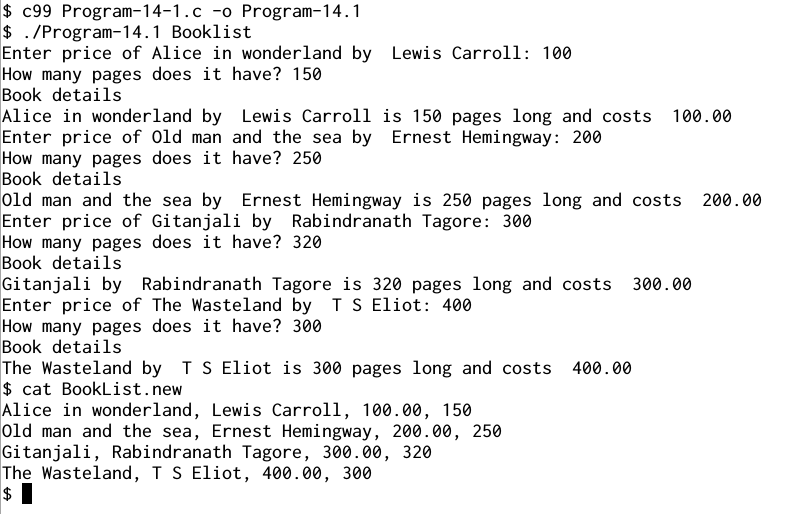
\includegraphics[scale=0.5]{Output-14-1.png}
\caption{Using structures}
\label{output-14-1}
\end{center}
\end{figure}

\section*{Unions}
A \lstinline!union! is a special data type available in C that enables you to store different data types in the same memory location. You can define a union with many members, but only one member can contain a value at any given time. Think of these members as synonyms for the same memory location; but with different syntax and semantics depending on their data type. 

\subsection*{Defining a Union}
To define a union, you must use the union statement. The union statement defines a new data type, with more than one member for your program.

The format of defining union  is as follows:
\begin{lstlisting}[numbers=none]
    union <union_name> {
        member definition;
        member definition;
             ...
        member definition;
    } [one or more union variables];
\end{lstlisting}

Here is the way you would define a \lstinline!union! named \emph{data} which has the three members i, f, and str of int, float and char array.
\begin{lstlisting}[numbers=none]
  union data_t {
    int i;
    float f;
    char str[20];
  } data; 
\end{lstlisting}

Now, a variable of \lstinline!data_t! type can store an integer, OR a floating-point number, OR a string of characters. This means that the same memory location can be used to store multiple types of data. You can use any built-in or user defined data types inside a union based on your requirement.

To access any member of a union, we use the member access operator (.), similar to structures. 

\texttt{union\_variable.union\_member}

\subsection*{Union vs Structure}
The differences between structure and union are: 
\begin{itemize}
\item union allocates the memory equal to the memory required by the largest member of the union but structure allocates the memory equal to the total memory required by all the members. 
\item In union, one memory block is used by all the member of the union but in case of structure, each member have their own memory space.
\item structure enables us to treat a collection of number of data items as a single composite entity, a union enables us to look at the same space in memory in one of many different ways.
\end{itemize}

\section*{Arrays of Structure}
Structure is used to store the information of one particular object but if we need to store 100 such objects then Array of Structure is used. Since structures are like any other data type it is easy to understand the declaration, definition and usage.

\begin{lstlisting}[numbers=none]
  struct book_t {
    char title[25];
    char author[40];
    float price;
    int pages;
  } library[100];
\end{lstlisting}

OR 

\begin{lstlisting}[numbers=none]
  struct book_t {
    char title[25];
    char author[40];
    float price;
    int pages;
  };
  ....
 struct book_t library[100];
\end{lstlisting}

Both are equivalent methods of declaring an array of 100 books called a library. Accessing an individual book in an array is by the usual array access mechanism: \texttt{library[n]} refers to the $(n + 1)^{th}$ element of the array. Accessing a member of a particular element is also as expected: \texttt{library[n].title} 

\section*{Pointers to Structures}
Like any other data item a structure variable also has an address and can be manipulated using pointers.

For example, continuing with the book, \lstinline!struct book_t* pBook;! defines a pointer to a structure. The way to initialize would be to take the address of a book\_t, for example: \texttt{pBook = \&mathBook;}

Referring to a member becomes a little tricky. \texttt{*pBook.title} will not work as the precedence of dot is higher; so you have to write \texttt{(*pBook).title}. There is an  alternative notation available, namely
\texttt{pBook->title}, and this definitely is better.
\end{document}